\section{Fremstilling}
\subsection{Projektiler}
Vi udformede projektilerne ved at benytte normale 40mm bordtennisbolde, hvor 3 blev overmalet med akrylmaling for at give dem stærk farve af hhv. rød, grøn og blå. Se Figur \ref{fig:akrylbolde} 
\begin{figure}[H]
	\centering
    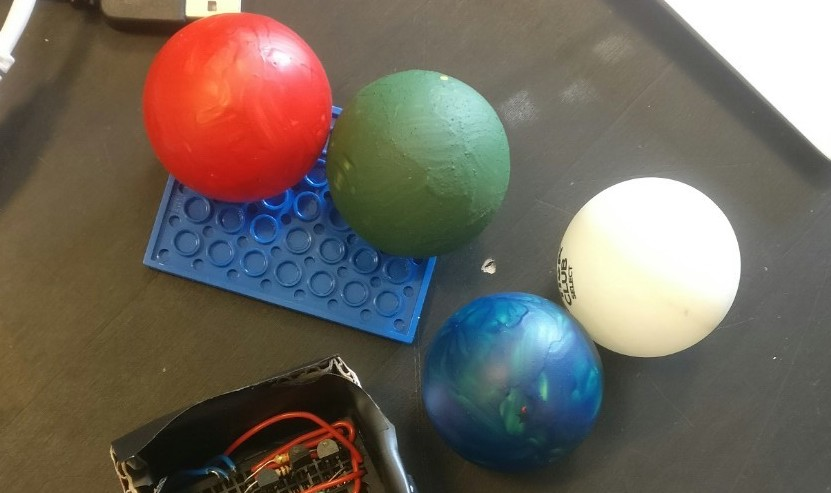
\includegraphics[width=13cm]{figures/2_5fremstilling/akrylbolde.jpeg}
	\caption{Et billede af vores benyttede projektiler}
	\label{fig:akrylbolde}
\end{figure}
\subsection{Fumlebræt-modeller}
Vi lavede en række fumlebrætsmodeller for forskellige dele af det samlede kredsløbet. 
	\begin{figure}[H]
		\centering
	    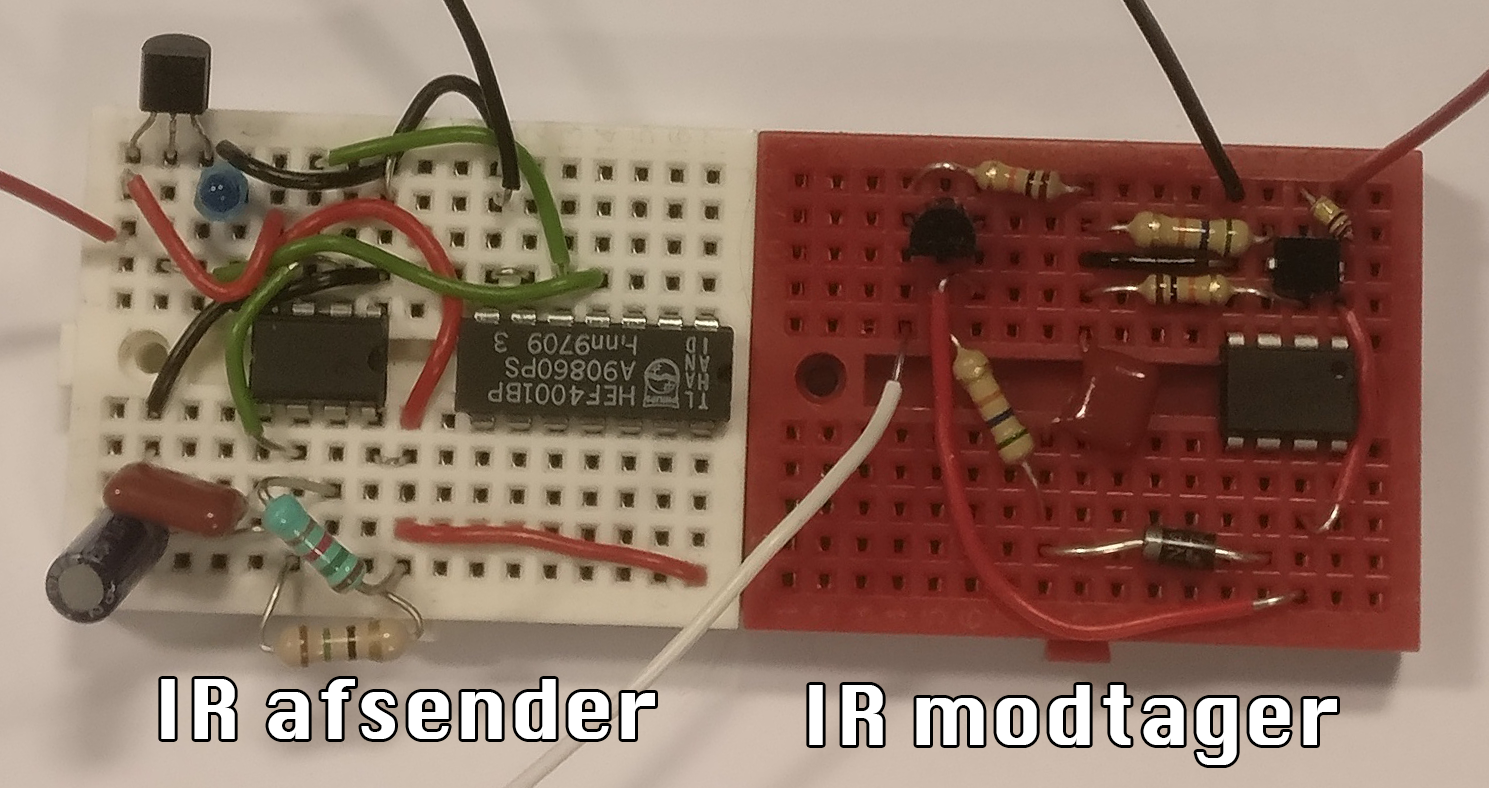
\includegraphics[width=13cm]{figures/2_5fremstilling/prototyper/DanielChrisKreds.png}
		\caption{}
		\label{fig:}
	\end{figure}
\subsection{PCB - fremstilling}\label{subs:pcbfremstilling}
Vi ønskede vores kredsløb på et par mindre PCB. Vi designede to PCB i programmet Livewire i kombination med PCB Wizard. Det ene PCB havde 4 delkredse som skulle skilles fra hinanden ved savning. Disse delkredse var 2 af dem IR-afsender kredsløbet og 2 af dem var IR-modtager kredsløbet. Se det første PCB i Bilag \ref{bilag:afsenderModtagerArtwork}. 

Det andet PCB var et shield til arduinoen der skulle forbindes til diverse kredsløb. Se Bilag \ref{bilag:shieldArtwork}.
\subsubsection{Kemisk fremstilling}
Ved at printe vores print på transfer-papir, kan det benyttes som beskyttelse på kobberplader. Kobberpladerne bliver først UV-belyst, hvor de derefter skylles i en blanding af vand og kaustisk soda indtil printet kan tydeligt ses. Herefter skylles kobberpladen og den lægges i et syrekar indtil de ubeskyttede områder er tilstrækkeligt ætset væk.

\subsubsection{Problemer med printboards}
\todo{Beskriv hvordan PCB-baseret produkt ikke fungrede, har vi nogen mulige forklaringer?} 
Vi havde produceret 3 forskellige printboards som vi prøvede at få til at virke.
På det først bræt var det ikke alle steder hvor syren havde ætset kopperet væk i den kemiske fremstillingsfase, hvilket kunne være medførst af at syren ikke blev fordelt ordenligt da den skulle i syrebadet.
med vores næste forsøg blev der brugt en for høj varme til at lodde de forskellige komponeter på at noget af kopper blev loddet af sammen med det. Dette kunne nemt blive undgået ved at man fremover kun bruger temperature der skal til for at smelte lige netop den type af loddetin der blev brugt til vores produkt.
På det sisdte har det været meget svært at se en tydelig fejl da alle de forskellige tænkelige problemer der kunne medføre at det ikke virker er blevet testet. 
Test 1 har været at der muligvis har været forbindelse forskellige steder på vores PCB. Dette blev dog testet ved at bruge et multimeter og teste for kortslutninger.
Test 2 har været at der muligvis manglede ledninger på selve PCB layoutet. Der er stor mulighed for at der er nogle ledninger der ikke bliver placeret i PCB-wizard hvis man laver manuelle ændringer som vi har gjort for at placere 4 forskkellige dele overskueligt på PCBet. Vi har dog gjort en betydelig insats for at dette ikke bliver et problem ved bare at lave det med så få menneskelige inflydelse som muligt. og ved at checke det igennem bagefter.
test 3 som er at der er noget galt med nogle af komponenterne. Der er forskellige ting som kunne være skyld i dette. De kunne være placeret med forkert rotation eller at der er brugt forkerte komponenter eller det kunne være muligt at der er nogle af komponenterne der simpelhen ikke virker. Vi har dog prøvet at kigge på komponenterne og se om der står det samme på dem som der gjorde i vores forrige prototybe, og det er ikke særlig ofte at komponenter ikke virker når de bliver insat i vores kredsløb. Men hvis vi selv har været skyld i at de ikke virker længere af forskellige årsager er det stædig det problem vi mener har størst mulighed for at være skyld i problemet af de overfor nævte mulige problemer.

\subsection{Endelige prototype}\label{subs:endeligProto}
\begin{figure}[H]
	\centering
    
\includegraphics[width=13cm]{figures/stock.jpg}
	\caption{Billede af endelig produkt}
	\label{fig:endeligPrototype}
\end{figure}




